\chapter{Basics and notation} 
In this chapter we introduce some basic notions that we shall use throughout this
Thesis. They include special property of trees, basic concepts for the nodes in trees and more evolved notations that will be needed in later section of this Thesis 
\section{Basic Graph Theoretic Concepts}
\begin{defin}
Let $T=(V,E)$ be a (simple) graph. $T$ is called a tree if it is connected and acyclic, meaning that for any pair of vertices $v \neq w \in V$ there exists exactly one path that has $v$ and $w$ as its endpoints. $T$ is called \textit{rooted} if one node $r \in V$ is designated as the root of the tree. $T$ is a \textit{labelled} tree, if there exists a labelling function $l:\;V\mapsto \Sigma$, where $\Sigma$ is an arbitrary set of labels.
\end{defin}
\begin{figure}[h!]
	\centering
    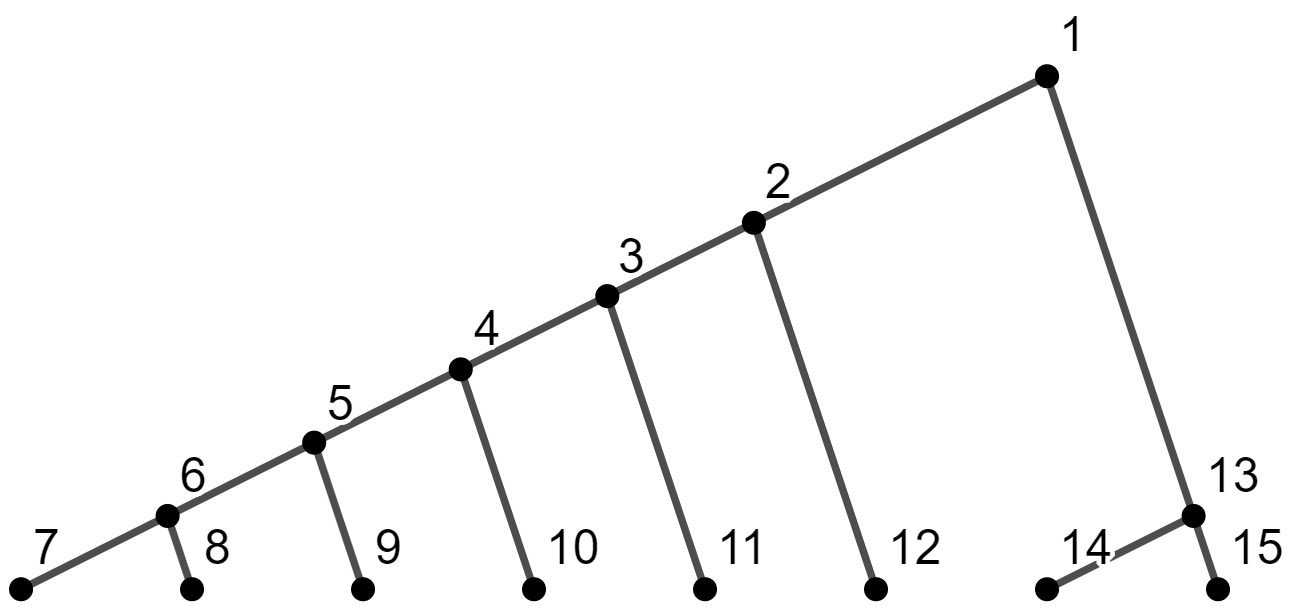
\includegraphics[width=0.6\textwidth]{figures/rooted_tree.jpg}
    \captionsetup{singlelinecheck=off}
    \caption{The illustration suggests, that the node $1$ is the root of the tree. Together with some function $l:\;\{1,..15\} \mapsto \{A,B,C\}$ $T$ is a rooted labelled tree.} \end{figure}
\begin{defin}
Let $T=(V,E)$ be a rooted labelled tree with root $r\in V$. We define the \textit{parent} $P(v) \in V$ of a node $v\in V\setminus \{r\}$ to be direct predecessor of $v$ on the unique path from $r$ to $v$ in $T$. The parent of $r$ is undefined. 
\end{defin}
\begin{defin}
Let $T=(V,E)$ be a rooted labelled tree with root $r\in V$, let $w,v \in V$. The node $w$ is a \textit{child} of $v$ if and only if $v$ is the parent of $w$. We denote by $C_T(v)$ the \textit{set of all children} of $v$:
$$ C_T(v):= \{w \in V | P(w) = v\}.$$
If the setting is clear one can use the shortcut $C(v)$ for $C_T(v)$
\end{defin}
\begin{defin}
Let $T=(V,E)$ be a rooted labelled tree with root $r\in V$, let $w \neq v \in V\setminus \{r\}$. The node $w$ is a sibling of $v$ if and only if $P(v) = P(w)$. We denote by $S(v)$ the \textit{sibling group of v}:
$$ S(v) := \{w \in V | P(w) = P(v)\}.$$
For the special case of the root $r$ we define the sibling group manually by $S(r) := \{r\}$.
\end{defin}
\begin{rem}
Note that for a node $v$ the following inclusion holds naturally:
$$v \in S(v)$$
That also implies that $|S(v)| >=1$.
\end{rem}
\begin{defin}
Let $T=(V,E)$ be a rooted tree. We call $T$ \textit{ordered} if all siblings have a specific and fixed order among each other. 
\end{defin}
\begin{figure}[h!]
	\begin{center} 
		\begin{tabular}{c}
		\xymatrix @R=4mm @C=2mm{
			&T_1&&&&&&T_2&\\
			&*+[o][F-]{A}\ar@{-}[dl]\ar@{-}[dr]&&&&&&*+[o][F-]{A}\ar@{-}[dl]\ar@{-}[dr]&\\
			*+[o][F-]{B}&&*+[o][F-]{C}&&&&*+[o][F-]{C}&&*+[o][F-]{B}
			}
		\end{tabular}
		\caption{If we assume that $T_1$ and $T_2$ are unordered trees, then $T_1 = T_2$. But if we consider them to be ordered from left to right as in the figure, then $T_1 \neq T_2$.}
	\end{center}
\end{figure}
\begin{defin}
Let $T=(V,E)$ be a rooted ordered tree with root $r\in V$ and let $n:= |V|$. The \textit{post-order index} is a way of enumerating the nodes of $T$ from $1$ to $n$. For that, you perform the following routine recursively starting with $v=r$ and index $m=1$:\\
\end{defin}\newpage
\begin{algorithm} % enter the algorithm environment
\caption{Assign the \textit{post-order} index to a tree $T$} % give the algorithm a caption
\label{alg1} % and a label for \ref{} commands later in the document
\begin{algorithmic}
\Function{Routine}{$v$, $m$}  
\If {($v$ is a leave) or (all children of $v$ are indexed)}
	\State Index $v$ with the index $m$;
	\State \Call{Routine}{$P(v)$, $m+1$}
\Else 
	\State Let $w$ be the left-most child of $v$ that has not yet been indexed.
	\State \Call{Routine}{$w$,$m$};
\EndIf
\EndFunction
\end{algorithmic}
\end{algorithm}
\begin{figure}[!ht]
	\begin{displaymath}
	\xymatrix @R=3mm @C=3mm{
		&&&T&&&\\
		&&&*+[o][F-]{13}\ar@{-}[d] &&&\\
		&&&*+[o][F-]{12}\ar@{-}[d] \ar@{-}[dll] \ar@{-}[drr]&&\\
		&*+[o][F-]{5} \ar@{-}[d]&&*+[o][F-]{6}&&*+[o][F-]{11} \ar@{-}[d]\\
		&*+[o][F-]{4} \ar@{-}[dl] \ar@{-}[d] \ar@{-}[dr]&&&&*+[o][F-]{10} \ar@{-}[dl] \ar@{-}[d] \ar@{-}[dr]\\
		*+[o][F-]{1}&*+[o][F-]{2}&*+[o][F-]{3}&&*+[o][F-]{7}&*+[o][F-]{8}&*+[o][F-]{9}	
	}
	\end{displaymath}
	\caption{An example of the post order indexing. Note that for every subtree the root is indexed at last.}
	\label{fig:postorder}
\end{figure} 
\begin{defin} Let $T=(V,E)$ be an ordered tree rooted at $r \in V$. If $|V| > 1$ we denote by $T^{\circ} := T \setminus \{r\}$ be the forest, which results from $T$ after deleting the root $r$. Moreover for a node $v\in V$ we denote by $F_v$ the subtree of $T$ rooted at $v$. 
\end{defin}
\begin{defin} Let $T=(V,E)$ be an ordered forest. We denote by $L_T$ and $R_T$ the left- and rightmost subtrees of $T$ respectively. Furthermore the roots of $L_T$ and $R_T$ are denoted by $l_T$ and $r_T$ respectively
\end{defin}
\begin{rem}
Consider the tree $T$ in Figure~\ref{fig:postorder}. Then we can use the notion introduced above to describe the following trees:
\begin{figure}[!ht]
	\begin{subfigure}[b]{0.49\textwidth}
	\caption{$T^{\circ}$}
	\begin{displaymath}
	\xymatrix @R=3mm @C=3mm{
		&&&*+[o][F-]{12}\ar@{-}[d] \ar@{-}[dll] \ar@{-}[drr]&&\\
		&*+[o][F-]{5} \ar@{-}[d]&&*+[o][F-]{6}&&*+[o][F-]{11} \ar@{-}[d]\\
		&*+[o][F-]{4} \ar@{-}[dl] \ar@{-}[d] \ar@{-}[dr]&&&&*+[o][F-]{10} \ar@{-}[dl] \ar@{-}[d] \ar@{-}[dr]\\
		*+[o][F-]{1}&*+[o][F-]{2}&*+[o][F-]{3}&&*+[o][F-]{7}&*+[o][F-]{8}&*+[o][F-]{9}	
	}
	\end{displaymath}
	\end{subfigure}
	\begin{subfigure}[b]{0.49\textwidth}
	\caption{$T_{12}^{\circ}$}
	\begin{displaymath}
	\xymatrix @R=3mm @C=3mm{
		&*+[o][F-]{5} \ar@{-}[d]&&*+[o][F-]{6}&&*+[o][F-]{11} \ar@{-}[d]\\
		&*+[o][F-]{4} \ar@{-}[dl] \ar@{-}[d] \ar@{-}[dr]&&&&*+[o][F-]{10} \ar@{-}[dl] \ar@{-}[d] \ar@{-}[dr]\\
		*+[o][F-]{1}&*+[o][F-]{2}&*+[o][F-]{3}&&*+[o][F-]{7}&*+[o][F-]{8}&*+[o][F-]{9}	
	}
	\end{displaymath}
	\end{subfigure}
	\begin{subfigure}[b]{0.32\textwidth}
	\caption{$L_{T_{12}^{\circ}} = T_5$}
	\begin{displaymath}
	\xymatrix @R=3mm @C=3mm{
		&*+[o][F-]{5} \ar@{-}[d]&\\
		&*+[o][F-]{4} \ar@{-}[dl] \ar@{-}[d] \ar@{-}[dr]&\\
		*+[o][F-]{1}&*+[o][F-]{2}&*+[o][F-]{3}&
	}
	\end{displaymath}
	\end{subfigure}
	\begin{subfigure}[b]{0.32\textwidth}
	\caption{$R_{T_{12}^{\circ}} = T_{11}$}
	\begin{displaymath}
	\xymatrix @R=3mm @C=3mm{
		&*+[o][F-]{11} \ar@{-}[d]\\
		&*+[o][F-]{10} \ar@{-}[dl] \ar@{-}[d] \ar@{-}[dr]\\
		*+[o][F-]{7}&*+[o][F-]{8}&*+[o][F-]{9}	
	}
	\end{displaymath}
	\end{subfigure}
	\begin{subfigure}[b]{0.32\textwidth}
	\caption{$R_{T_{12}^{\circ}}^{\circ} = T_{11}^{\circ} = T_{10}$}
	\begin{displaymath}
	\xymatrix @R=3mm @C=3mm{
		&*+[o][F-]{10} \ar@{-}[dl] \ar@{-}[d] \ar@{-}[dr]\\
		*+[o][F-]{7}&*+[o][F-]{8}&*+[o][F-]{9}	
	}
	\end{displaymath}
	\end{subfigure}
	\caption{Different subtrees using the introduced notion.}
	\label{fig:subtrees}
\end{figure} 
\end{rem}
\begin{defin} Let $T_i=(V_i,E_i)$ be a rooted tree. We call $t_i:= |V_i|$ the size of the tree $T_i$. Furthermore we use the notion of $t_{l,i}$ for the number of leaves in $T_i$ and $t_{h,i}$ for the length of the longest path from the root to any leaf. 
\end{defin}
\begin{rem}
We will need this definitions mainly for stating the running times of algorithms. Since we want to compare $T_1$ with $T_2$ we need to be able to separate those numbers accordingly. Furthermore, if a tree is significantly bigger, we always assume that tree $T_1$ is the bigger one, i.e. $\mathcal{O}(t_1)\geq \mathcal{O}(t_2)$.
\end{rem}
\begin{defin}
Let $T$ be a forest which is ordered according to the post order indexing. Let $T'$, $T''$ be two induced subforests of $T$ with $\exists i_{T'},j_{T'},i_{T''},j_{T''}$ s.t. $V(T')=\{i_{T'},...,j_{T'}\}$ and $V(T'')=\{i_{T''},...,j_{T''}\}$.\\
We call $T'$ to a \textit{prefix} of $T''$ if and only if the following holds:
$$i_{T'} = i_{T''} \quad \text{and} \quad j_{T'} \leq j_{T''}$$
\end{defin}
\begin{defin}
Let $T$ be an ordered tree rooted at $r$. Then we define the \textit{keyroots} of $T$ to be set of all nodes that have a left sibling:
$$\text{keyroots}(T) := \{r\} \cup \{v \in V(T) \,|\,v\text{ has a left sibling}\}.$$\\
Assume $T$ is an ordered forest with trees $T_1,...,T_n$ rooted at $r_1,...r_n$. Then we define the set of keyroots as the union of the separated sets of keyroots:
$$\text{keyroots}(T) = \sideset{}{}\bigcup_{i=1}^n \text{keyroots}(T_i).$$
\end{defin}
\begin{defin}
Let $T$ be an ordered tree rooted at $r$. For a node $v$ we define the \textit{collapse depth} of $v$ cdepth$(v)$ to be the number of keyroot ancestors of $V$:
$$\text{cdepth}(v) = |\{w \in V(T)\,|\, w \text{ is an ancestor of }v\} \cap \text{keyroots}(T)|.$$
\end{defin}
\begin{defin}
Let $T$ be an ordered tree rooted at $r$. For every non-leaf node $n$ we choose one node $m \in C(n)$ among those with the most descendants in $C(n)$ arbitrarily. We define $m$ to be a heavy node. All non-heavy nodes are defined as \textit{light}, especially the root $r$. 
\end{defin}
\begin{rem}
In most cases a tree has multiple possibilities for the definition of heavy nodes. For example if there are multiple leaves with the same parent.
\end{rem}
\begin{defin}
Let $T$ be an ordered tree rooted at $r$ and let there be a fixed definition of heavy nodes. We call an edge to be \textit{heavy} if it connects a non-leaf with its heavy child. Furthermore we call a path, which connects a light node with a leaf and only consists of heavy edges a heavy path. We call the heavy path originating at the root $r$ the \textit{main heavy path}. The set of all heavy paths is called a \textit{heavy path decomposition}. 
\end{defin}
\begin{rem}
Light leaves are a special case of heavy paths of length 0.
\end{rem}
\begin{rem}
The heavy path decomposition depends on the choice of heavy nodes.
\end{rem}
\begin{figure}[!ht]
	\centering
	\begin{subfigure}[b]{0.45\textwidth}
	\caption{}
	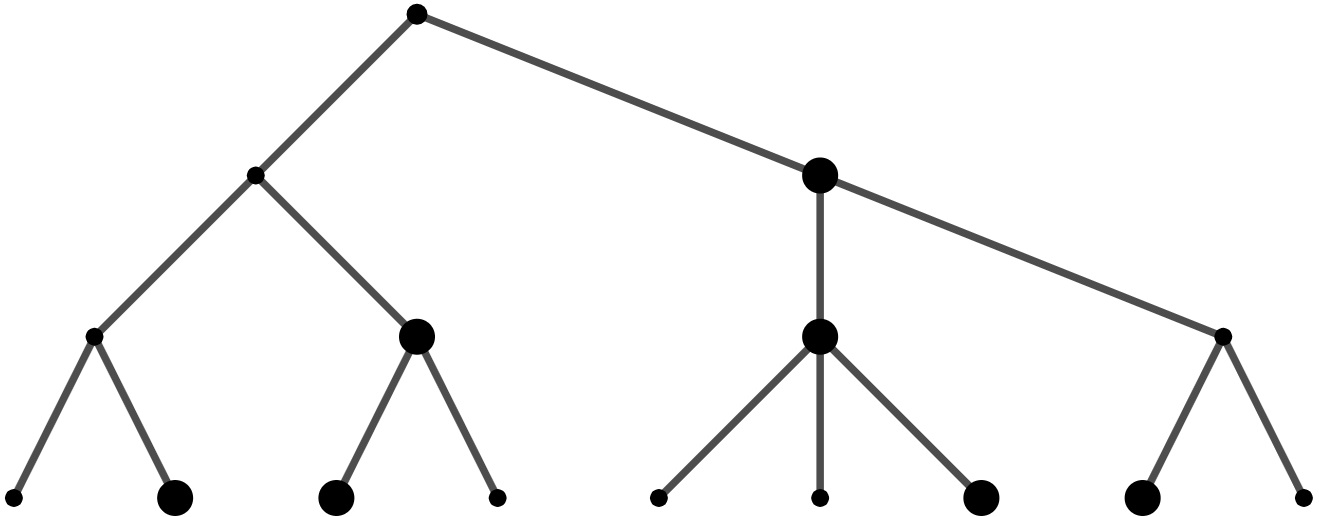
\includegraphics[width=\textwidth]{figures/heavy_nodes.jpg}
    \end{subfigure}
    \begin{subfigure}[b]{0.45\textwidth}
	\caption{}
	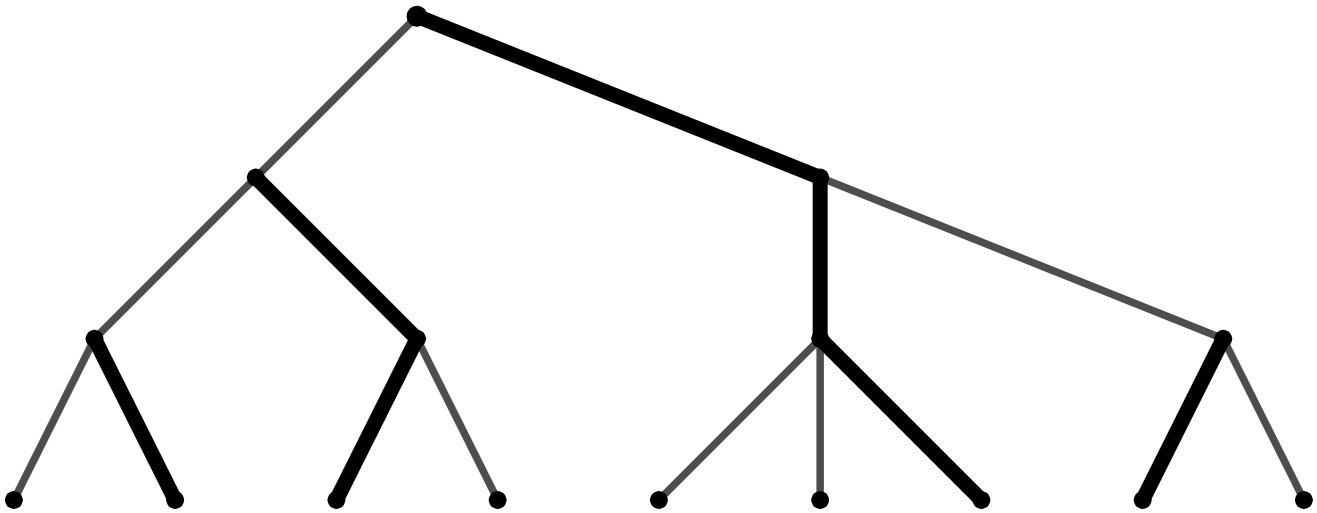
\includegraphics[width=\textwidth]{figures/heavy_path_decomposition.jpg}
    \end{subfigure}
	\caption{Example of a heavy path decomposition. Figure a) shows the heavy nodes, Figure b) the correspondig heavy paths.}\label{fig:heavypath}
\end{figure}
\begin{defin}
Let $T$ be an ordered tree rooted at $r$, $v \in V(T)$ and suppose a heavy path decomposition is fixed. we define the \textit{light depth} ldepth$(v)$ to be the number of light proper ancestors of $v$.\\
Furthermore we define ldepth$(T)$ as follows:
$$\text{ldepth}(T) = \max \{\text{ldepth}(v) \,|\,v \in T\}.$$
\end{defin}
\begin{defin}
Let $T$ be an ordered tree rooted at $r$ and let a heavy path decomposition be given. We define the set TopLight$(T)$ to be the set of all light nodes $v \in V$ with ldepth$(v) = 1$:
$$\text{TopLight}(T) := \{v \,|\,\text{ldepth}(v)=1 \text{ and } v \text{ not in the main heavy path of }T\}.$$
\end{defin}
\begin{rem}
A light node $v\in V(T)$ is in TopLight$(T)$ if and only if its parent lies on the main heavy path of $T$.
\end{rem}
\begin{defin} Let $T$ be a tree, $X$ the set of leaves of $T$ and $\Sigma$ a set of labels. Then $T$ is an \textit{unrooted phylogenetic} tree if all leaves are labelled bijectively with some label in $\Sigma$, all interior leaves are unlabelled and all interior nodes have degree at least three. A \textit{rooted phylogenetic} tree is a phylogenetic tree where one node, the root $r \in V(T)$, is distinguished from the others and may have degree two.  
\end{defin}
\begin{defin} Let $T$ be a phylogenetic tree, $X$ the set of leaves of $T$ and $\Sigma$ the set of labels of $X$. Then $\Sigma$ is called the set of \textit{taxa}. 
\end{defin}
\begin{defin} Let $T$ be a phylogenetic tree and $X$ the set of leaves of $T$. Some $C \subset X$ is called a \textit{clade} if $\exists \,v \in T$ s.t. $C$ is the set of leaves in the induced subtree $T_v$ of $T$. A clade $C$ is called \textit{trivial} if $|C|=1$ or $C = X$. The set $\mathcal{C}(T) := \{C \subset V\;|\; C\text{ is a clade}\}$ is the set of clades of $T$, $\mathcal{C}^*(T) := \{C \in \mathcal{C}(T)\;|\; C\text{ is non trivial}\}$ the set of non trivial clades.
\end{defin}
\begin{defin} A rooted tree $T$ is called \textit{full binary}, if every node has either $0$ or $2$ children. 
\end{defin}
\begin{rem}
In some literature, a binary tree is defined as a tree, where every node has $\leq 2$ children. This contains the possibility of nodes having exactly $1$ child. In the context where we will use binary trees, this kind of behavior is not desired. Therefore we ensure all nodes to either be a leaf or have exactly $2$ children. This results in trees with a nice property: 
\begin{lem}
Let a full binary tree $T$ with $n$ leaves be given. Then $T$ has $2n-1$ nodes over all.
\end{lem}
\begin{proof}
We make an inductive argument. For $n \, \in \, \{0,1,2\}$ this is a trivial statement. Assume the statement holds $\forall \, m \leq n$.\\
$n \to  n+1$: Let $l$ be the left child and $r$ the right child of $T$'s root. Since $T$ is a full binary tree, $T_l$ and $T_r$ also have to be full binary trees. We define $m_l$ to be the number of leaves in $T_l$ and $m_r$ the number of leaves in $T_r$. 
\begin{align*}
\Rightarrow \, m_l + m_r &= n \\
\Rightarrow \, |V(T_l)| &= 2m_l -1, \; |V(T_r)| = 2m_r - 1\\
\Rightarrow \, |V(T)| &= |V(T_l)| + |V(T_r)| + 1  \\
 \, &= (2m_l -1) + (2m_r -1) +1 \\
 \, &= 2(m_l+m_r)-1 = 2n-1 
\end{align*}
\end{proof} 
So when we compare two full binary trees with the same number of leaves, we know that these trees have exactly the same number of leaves. 
\begin{figure}[h!]
	\centering
    \includegraphics[width=0.6\textwidth]{figures/_full_binaryTrees.png}
    \captionsetup{singlelinecheck=off}
    \caption{An illustration of two binary trees. In both trees all nodes have $\leq 2$ children. However, only $T_1$ is a full binary tree because no node has exactly $1$ child.} 
\end{figure}
\end{rem}

\section{Other necessary Tools}
\begin{defin}
Let $T=(V,E)$ be a rooted labelled tree. The so called \textit{basic tree edit operations} on $T$ are \textit{relabelling, inserting} and \textit{deleting}: 
\begin{enumerate}
\item \textit{Relabelling $v$:} changing the label of a node $v$.
\item \textit{Inserting $v$ underneath $v'$: } insert a new node $v$ into $T$ as a child of $v'$ and assign the children of $v'$ to the new node $v$. Denote the new tree by $T'$, then: 
$$C_{T'}(v') = \{v\}\text{ and }C_{T'}(v) = C_T(v')$$.
\item \textit{Deleting $v$ underneath $v'$: } the opposite transformation of inserting. Delete $v$, assign all children of $v$ to $v'$ in the same order. Denote the new tree by $T'$, then: 
$$C_{T'}(v') = C_T(v')\setminus \{v\} \cup C_T(v)$$.
\end{enumerate}
\end{defin}
\begin{figure}[b]
	\captionsetup[subfigure]{labelformat=empty}
	\centering
	\begin{subfigure}[b]{0.18\textwidth}
	\caption{}
	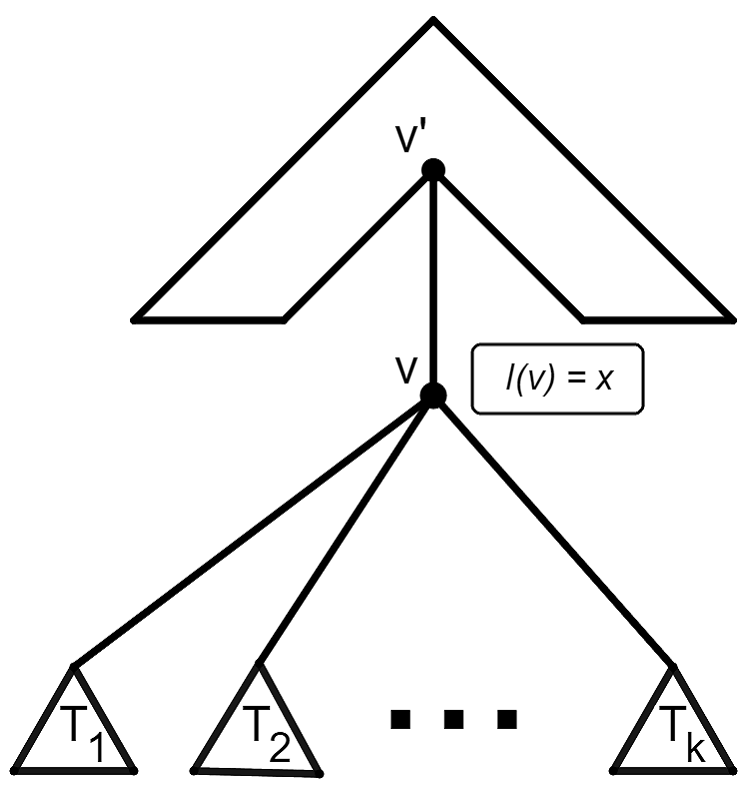
\includegraphics[width=\textwidth]{figures/TreeEditOperation_1.png}
    \end{subfigure}
    \begin{subfigure}[b]{0.18\textwidth}
	\caption{}
	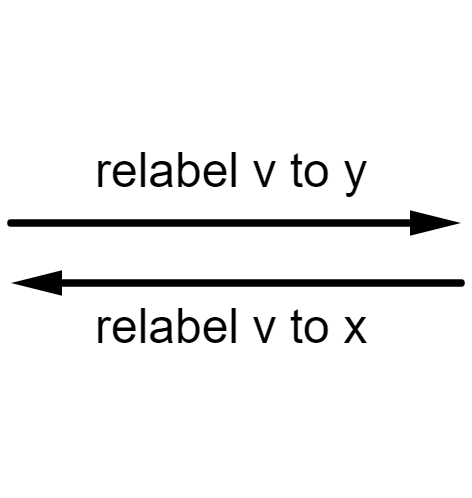
\includegraphics[width=\textwidth]{figures/TreeEditOperation_1,5.png}
    \end{subfigure}
    \begin{subfigure}[b]{0.18\textwidth}
	\caption{}
	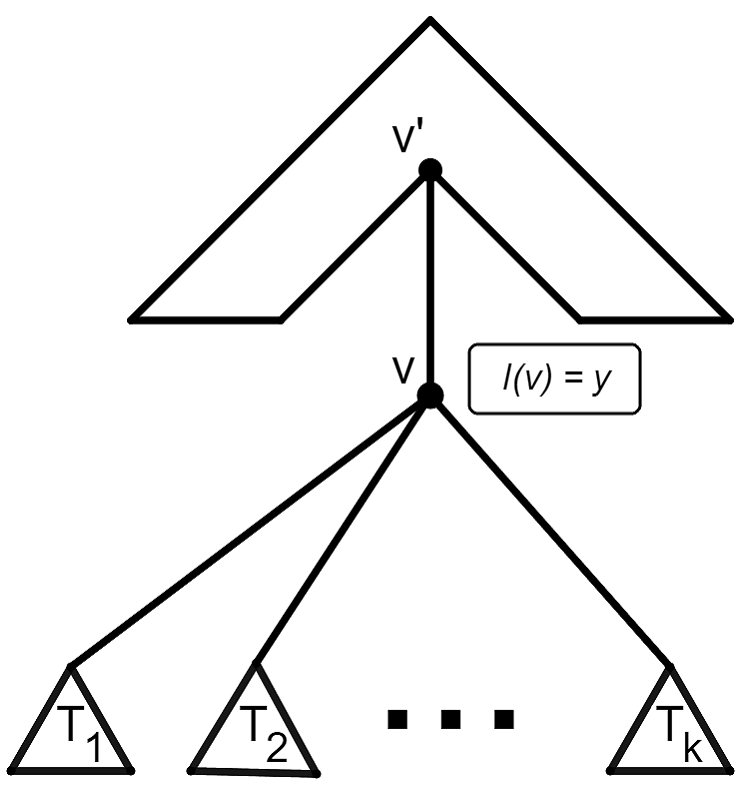
\includegraphics[width=\textwidth]{figures/TreeEditOperation_2.png}
    \end{subfigure}
    \begin{subfigure}[b]{0.18\textwidth}
	\caption{}
	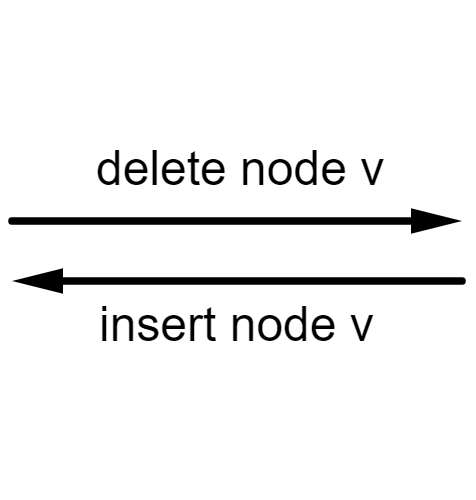
\includegraphics[width=\textwidth]{figures/TreeEditOperation_2,5.png}
    \end{subfigure}
    \begin{subfigure}[b]{0.18\textwidth}
	\caption{}
	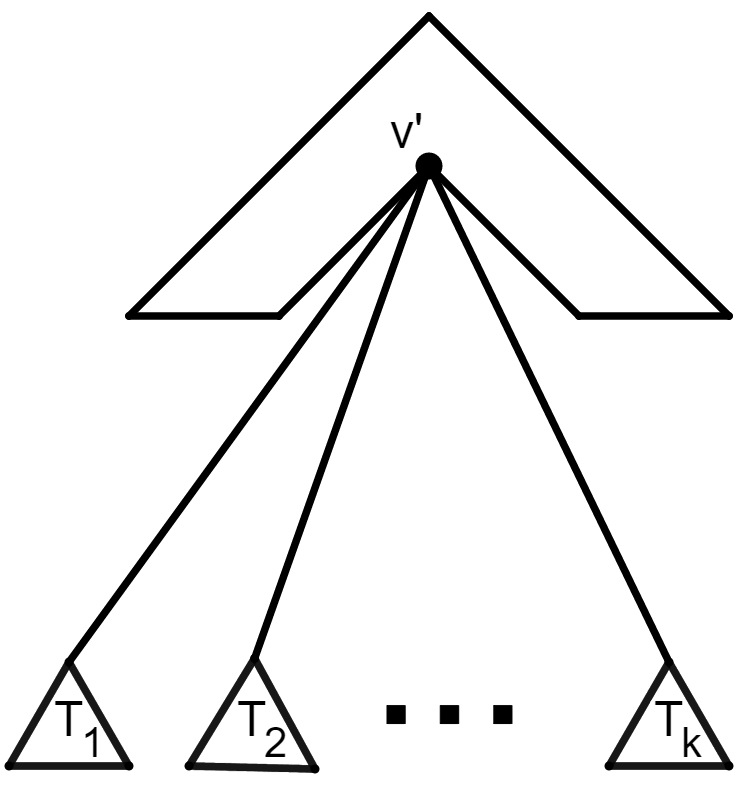
\includegraphics[width=\textwidth]{figures/TreeEditOperation_3.png}
    \end{subfigure}
	\caption{Illustration of the basic tree edit operations relabelling, deleting and inserting.}\label{fig:heavypath}
\end{figure}
\begin{defin}
Let $T=(V,E)$ be a rooted labelled tree and let $o$ be one of the basic edit operations defined above. We denote by $o(T)$ the tree that we get after executing the operation $o$ on the tree $T$. \\
Furthermore let $o'=(o'_1,o'_2,...,o'_n)$ be a finite sequence of basic edit operations. We define $o'(T)$ as the consecutive application of the basic operations:
$$o'(T) := o'_n(o'_{n-1}(...(o'_1(T)...)).$$
\end{defin}
\begin{defin}
Let $T=(V,E)$ be a rooted labelled tree, let $\Sigma$ be the set of labels and $\sigma, \sigma' \in \Sigma$. Furthermore let $o$ be one of the basic edit operations defined above. Then the cost of $c(o)$ is defined as:
\[
c(o) :=
\begin{dcases*}
        c_{rel}(\sigma, \sigma')  & Relabelling existing node $v$ from $\sigma$ to $\sigma'$\\
        c_{ins}(\sigma) & Inserting new node $v$ with label $\sigma$ \\
        c_{del}(\sigma) & Deleting existing node $v$ with label $\sigma$
\end{dcases*} 
\]
Moreover let $o'=(o'_1,...o'_n)$ be a finite sequence of basic edit operations. We define the costs of $o'$ to be the sum of costs of the individual operations:
$$c(o') := \sideset{}{}\sum_{i=1}^n c(o'_i).$$
\end{defin}
\begin{rem}
Because of the symmetry we can assume $c_{del}(\sigma) = c_{ins}(\sigma)$. Because of that, we will only work with relabelling and deleting operations later on.
\end{rem}
\begin{defin}
Let $T=(V,E)$ be a rooted labelled tree and let $o$ be one of the basic edit operations defined above. Then the cost of $c(o)$
\end{defin}
\begin{defin}
Let $T=(V,E)$ be a rooted labelled tree. A function $d: V\times V \mapsto \mathcal{R}$ is a \textit{metric} if the following conditions are fulfilled $\forall u,v,w, \in V$:
\begin{enumerate}
\item $d(v,w) \geq 0$
\item $d(v,w) = 0 \iff v=w$
\item $d(v,w) = d(w,v)$
\item $d(u,w) \leq d(u,v) + d(v,w)$
\end{enumerate}
\end{defin}

\begin{defin}
The \textit{Catalan numbers} $(C_n)_{n \in \mathbb{Z}_{\geq 0}}$ forms a sequence of natural numbers which occurs in many counting problems. They are recursively defined as follows:
\begin{align*}
C_0 &= 1 \\
C_n &= \sum_{i=0}^{n-1} \; C_i C_{n-i-1} \text{ for } n \geq 1 
\end{align*}
\end{defin}
\begin{rem}
The following two counting problems are examples in which the Catalan numbers occur:
\begin{itemize}
\item Counting the number of pairwise different expressions containing $n$ pairs of parentheses where any prefix of the expression contains at least as many opening parentheses "(" as closing ones ")".~\cite{Ste}
\item Counting the number of pairwise different full binary trees with $n+1$ leaves. 
\end{itemize}
\end{rem}
\begin{lem}\label{lem:binCat}
The number of pairwise different full binary trees with $n+1$ leaves is exactly the $n$th-Catalan number $C_n$.
\end{lem}
\begin{proof}
We prove this statement via an induction. For $n=0$ the statement is trivial. There is only $1$ tree with exactly $1$ leaf, which is a single node.\\
Before performing the induction step, we introduce a notation. Let $k,l \, \in \, \mathcal{Z}_{> 0}$, then we introduce the following function:
$$C(k,l) := \bigg| \bigg\{T\, \Big| \, \parbox[position]{0.6\textwidth}{$T$ is a full binary tree where the left subtree has $k$ leaves and the right one has $l$}\bigg\}\bigg|$$ 
For the induction step assume that the inductive statement holds true for all $m < n$. Let's count the number of trees with $n+1$ leaves. Let an integer $i \, \in \mathbb{Z}_{\geq 0}$, $i < n+1$ be given. The number of pairwise different full binary trees with $n+1$ leaves, where the left subtree has $i$ leaves is $C(i, n+1-i)$. Because of the induction step we can determine this number:
$$C(i,n+1-i)= C_{i-1}C_{n+1-i-1}$$
If we sum up all $C(i,n+1-i)$ over all possible $i$, then he get the number of all pairwise different full binary trees with $n+1$ leaves:
\begin{align*}
&|\{\text{full binary trees with $n+1$ leaves}\}| \\
&= \sum_{i=1}^{n} C(i, n+1-i) \\
&= \sum_{i=1}^{n} C_{i-1}C_{n-(i-1)-1} \\
&= \sum_{i=0}^{n-1} C_{i}C_{n-i-1} = C_n
\end{align*}
\end{proof}
